\documentclass[11pt]{book}
\usepackage{amsmath}
\usepackage{amsfonts}
\usepackage{amssymb}
\usepackage{graphicx}

\usepackage{caption}
\usepackage{subcaption}
\usepackage{a4wide}



\begin{document}
\chapter{Results}
\section{Set up}
We started our experiment with 4 wells containing 2mM IPTG and 4 wells containing 100 ng/ml aTc with glucose M9 and chloramphenicol. We then added another set of 8 wells containing the same content but making the amount half to the previous set. We repeated the process several times and thus achieve a concentration gradient of IPTG and aTc shown in figure (\ref{concGrad}). 

We also had two overnight cultures (ONC1 and ONC2) of \textit{E. Coli} bacteria where ONC1 and ONC2 were in \textit{green} and \textit{red} states respectively, and also with a wild type MG1655 bacteria. We inoculated the IPTG and aTc wells with these bacteria. 

\section{Optical density and growth rate measurement}
The data that was achieved from the experiment provided us with the optical density (OD)of the cultures showed in figure (\ref{concGrad}). We measured the OD of each cell over time to observe if it shows the exponential nature of the bacterial growth rate. Since linearity in the logarithm scale is equivalent to the  exponentiality in the usual scale, we generated a logarithmic plot against time for each well. Figure (\ref{ODLogPlot}) shows these plots in detail.

OD can be treated as a good measure of bacterial growth rate since it increases with the number of bacteria. We subtracted the OD containing no bacteria from OD's of all cultures and generated the plots1. 

It is noticeable that the concentration of IPTG in A1-B8 and E1-F8 wells did not affect the growth rate much. This is desirable because we put the wild type MG1655 bacteria there, which can grow irrespective of the supplied media. 

C1-D8 and G1-H8 wells, where we mixed the ONC1 and ONC2 bacteria respectively show a similar exponential growthrate at least up to 10000 seconds from the experiment started. However, we expected to see stiffer curves in the right portion of of the plot-grid and flatter in the left portion which would signify the concentration gradient of the medium. From our data, it is not very clear if the concentration gradient affected the growth-rate significantly. 



We applied a linear fit on each of these data-sets and quantified the growth-rate as the slope of the linear fit. 

\begin{figure}
\centering
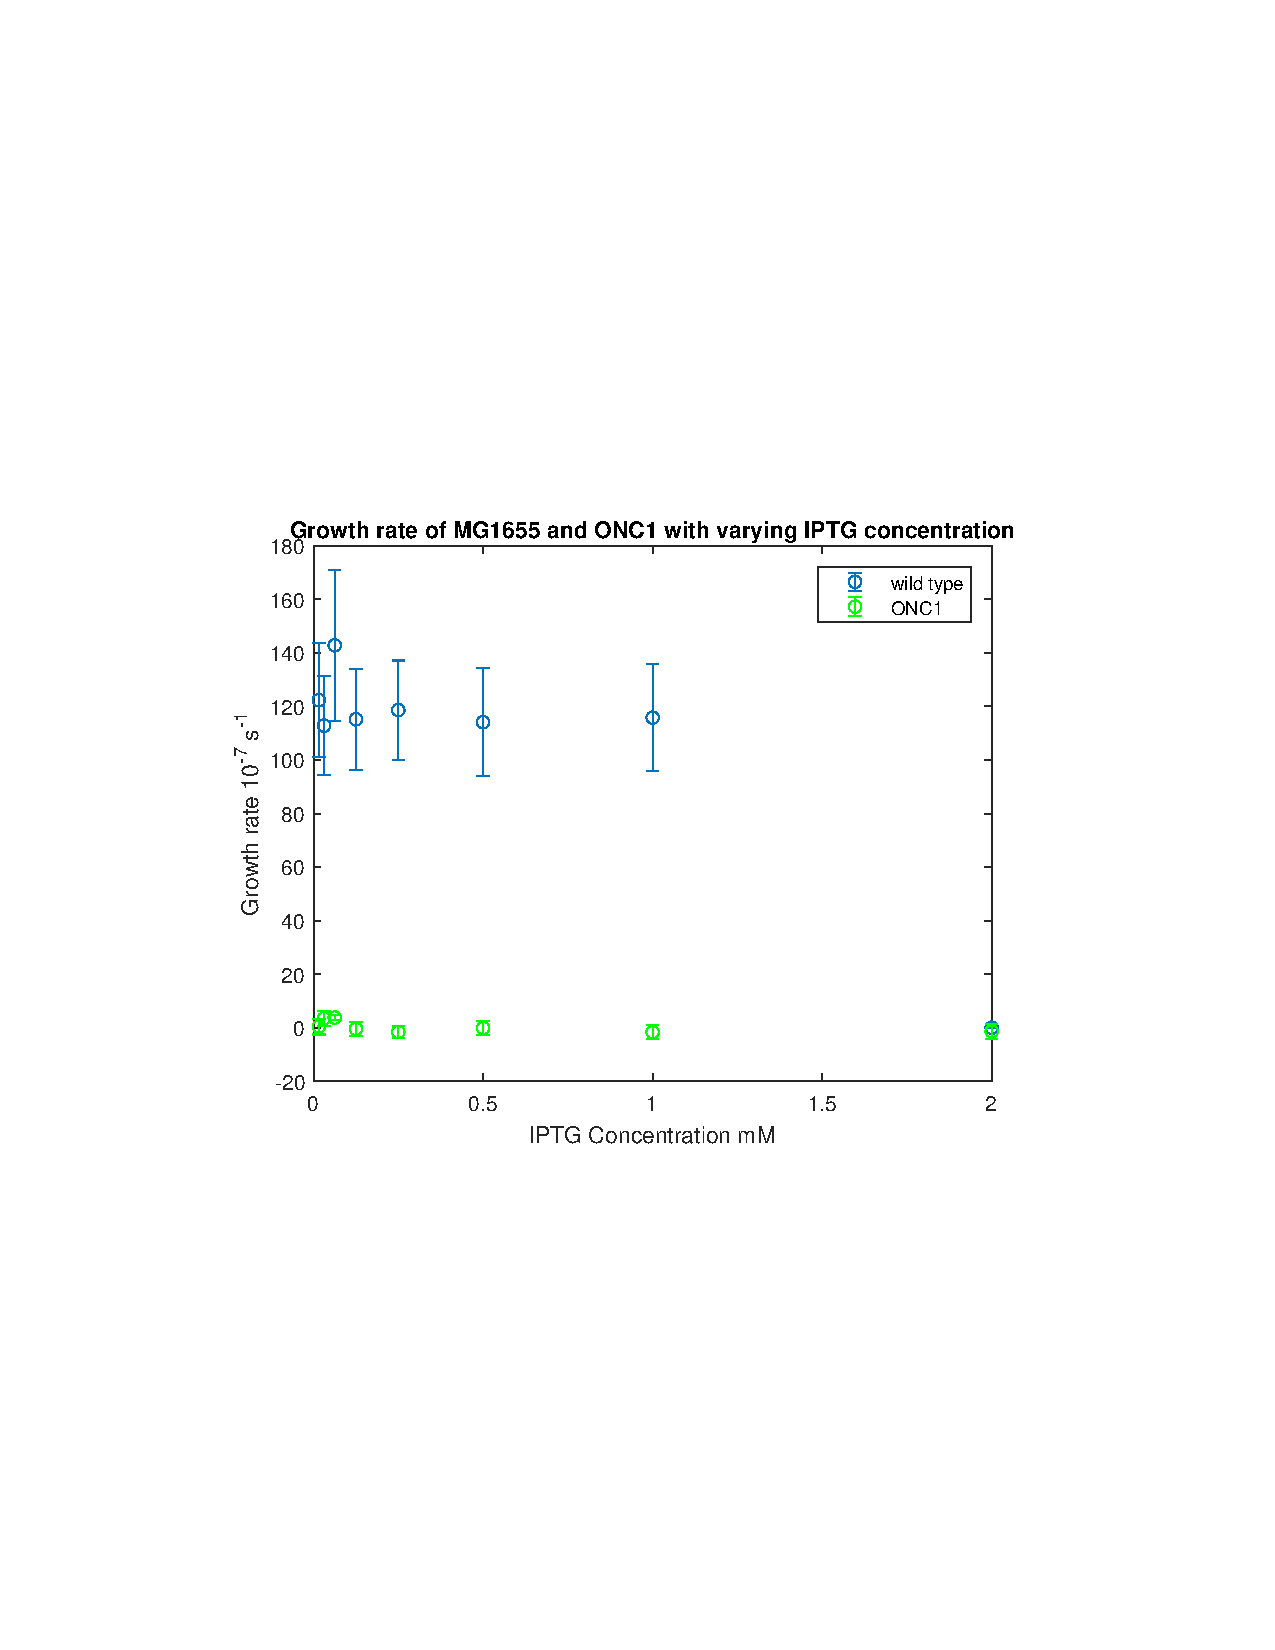
\includegraphics[scale=0.8]{ONC1growthrate.pdf}
\caption{ONC1}
\label{fig:GrowthrateODONC1}
\end{figure}

\begin{figure}
\centering
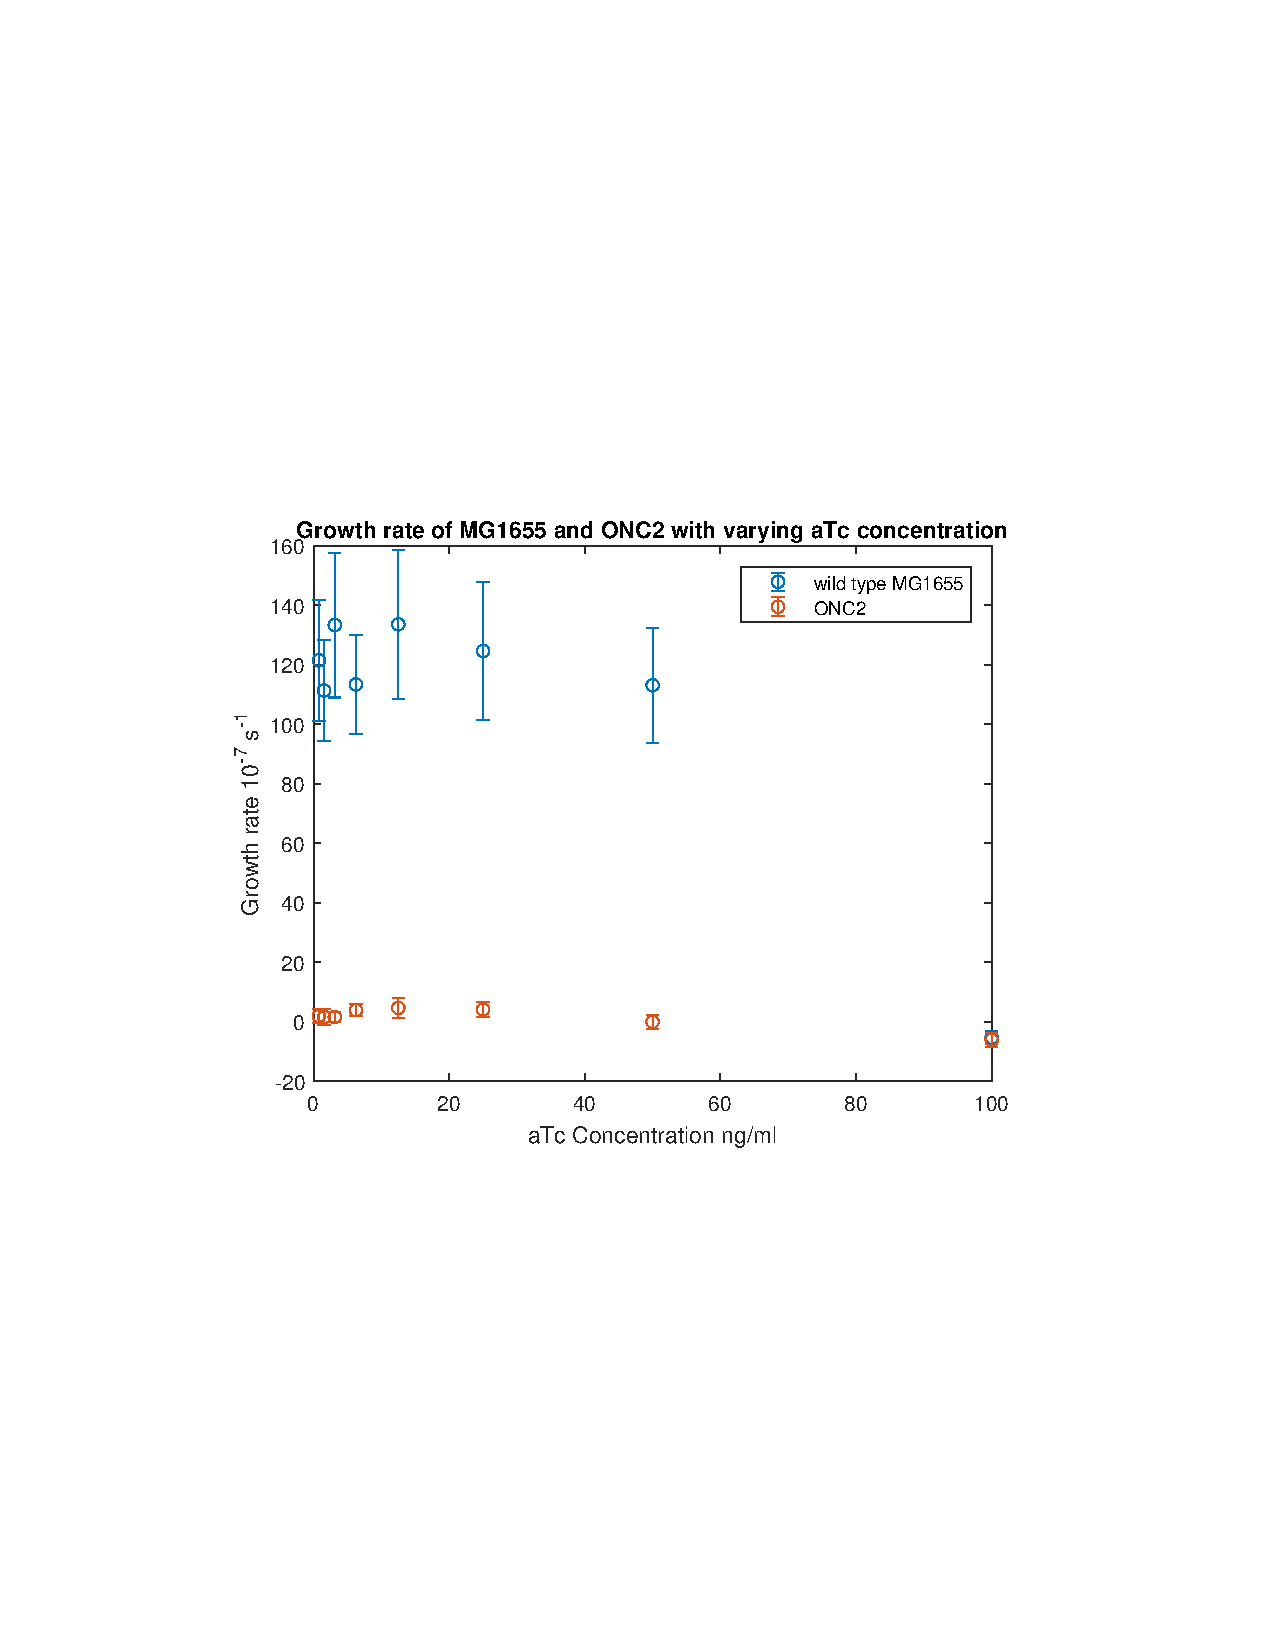
\includegraphics[scale=0.8]{ONC2growthrate.pdf}
\caption{ONC2}
\label{fig:GrowthrateODONC2}
\end{figure}

Figures \ref{fig:GrowthrateODONC1} and \ref{fig:GrowthrateODONC2} represent the plots of growth-rates at different time vs IPTG (or aTc) concentrations. We see that the data for wild type bacteria (denoted in blue) is consistent for the reason mentioned previously, where for the ONC's, it is not satisfactory. 

\section{GFP and RFP intensities and switching rate}
Besides OD, we also measured the fluorescence intensities of the green- and the red- fluorescent proteins (GFP and RFP) in the ONC1 and ONC2 respectively over time. The data for both are not initially comparable. So first we chose background intensities for each ONC's, subtracted them and normalized them by their intensities at initial values (at the beginning of the experiment). Figure \ref{fig:GfpRfpByOD} shows the details about this, where we plotted the GFP/OD and the RFP/OD (denoted green and red respectively) over time. Since OD can be also a good measure for cell-volume, hence GFP/OD and RFP/OD can be interpreted as fluorescence intensities per cell. 

Similar to the OD case, we applied an exponential fit (i.e. a linear fit with logarithmic vertical axis) on the GFP and RFP data and obtained the switching rates. 



\begin{figure}[h]
\centering
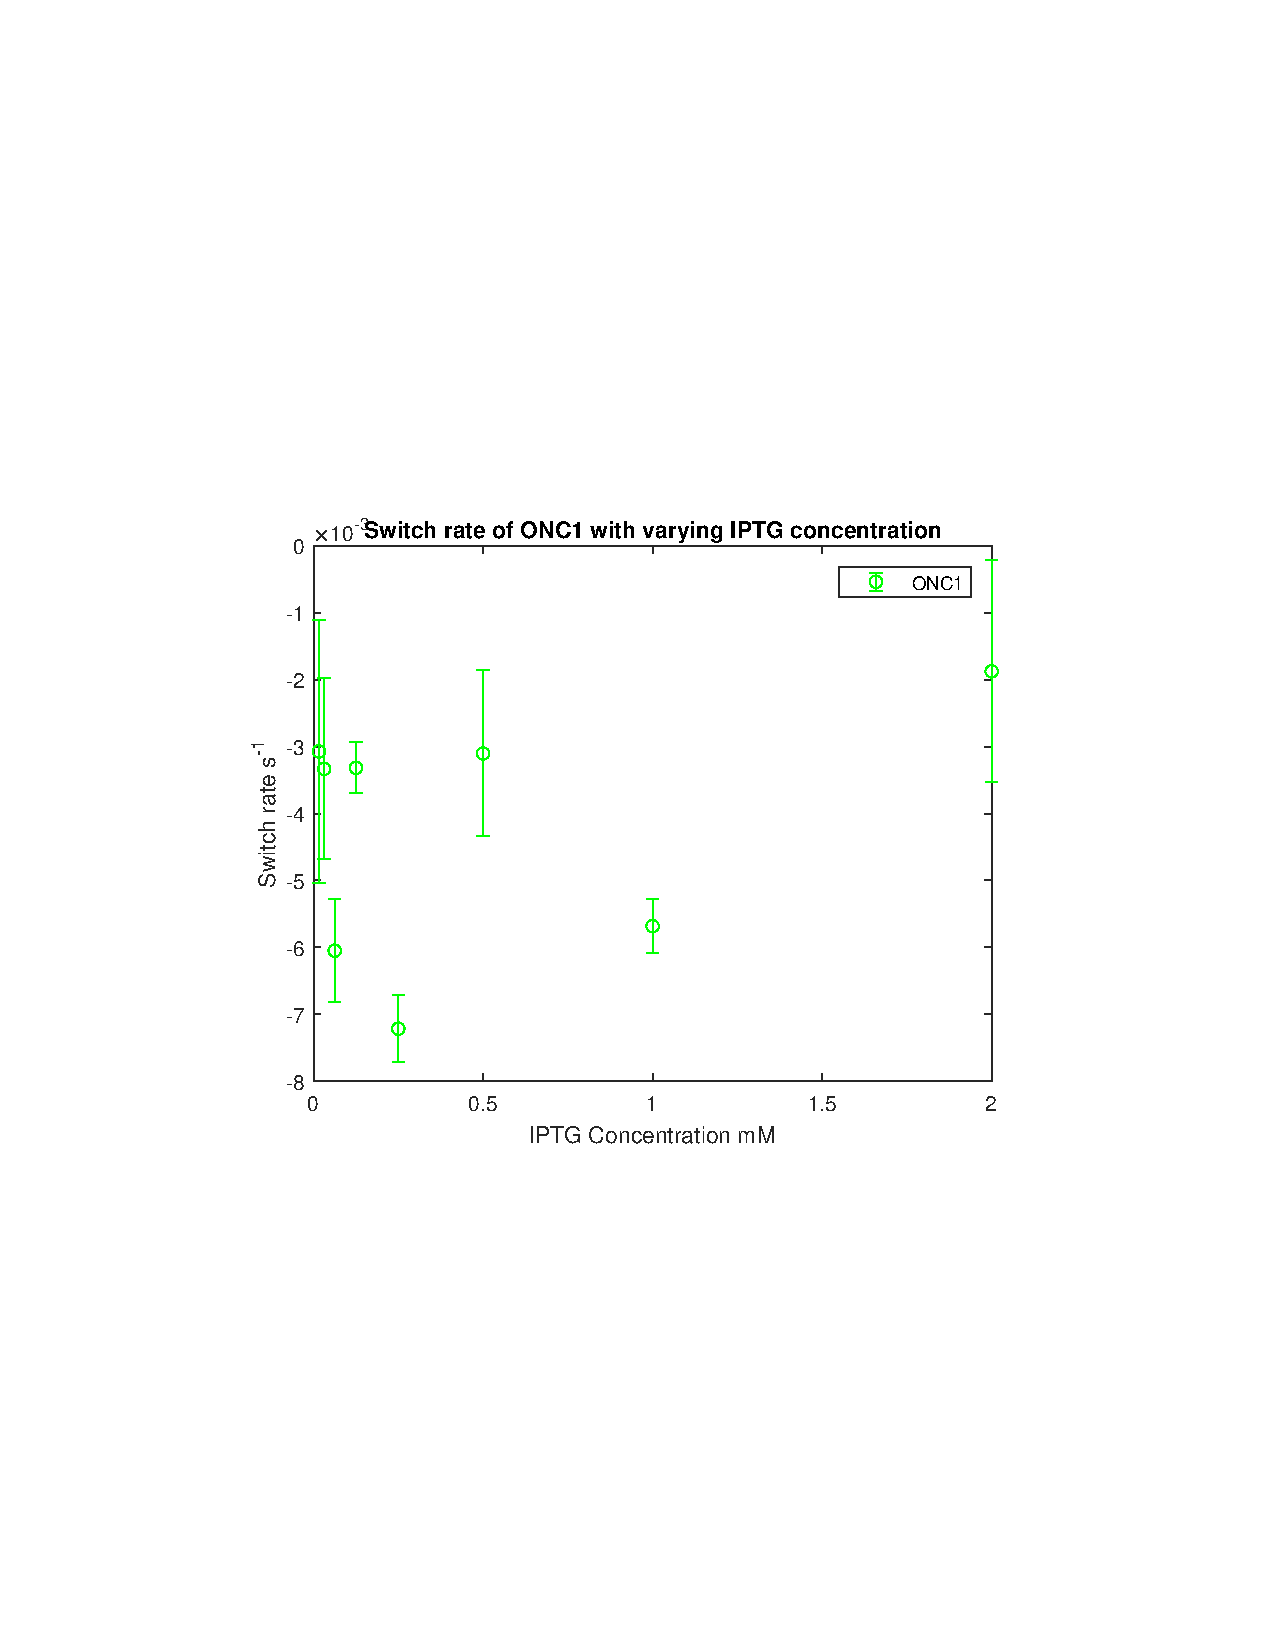
\includegraphics[scale=0.8]{ONC1switchrate.pdf}
\caption{}
\label{fig:onc1SwitchRate}
\end{figure}

\begin{figure}[h]
\centering
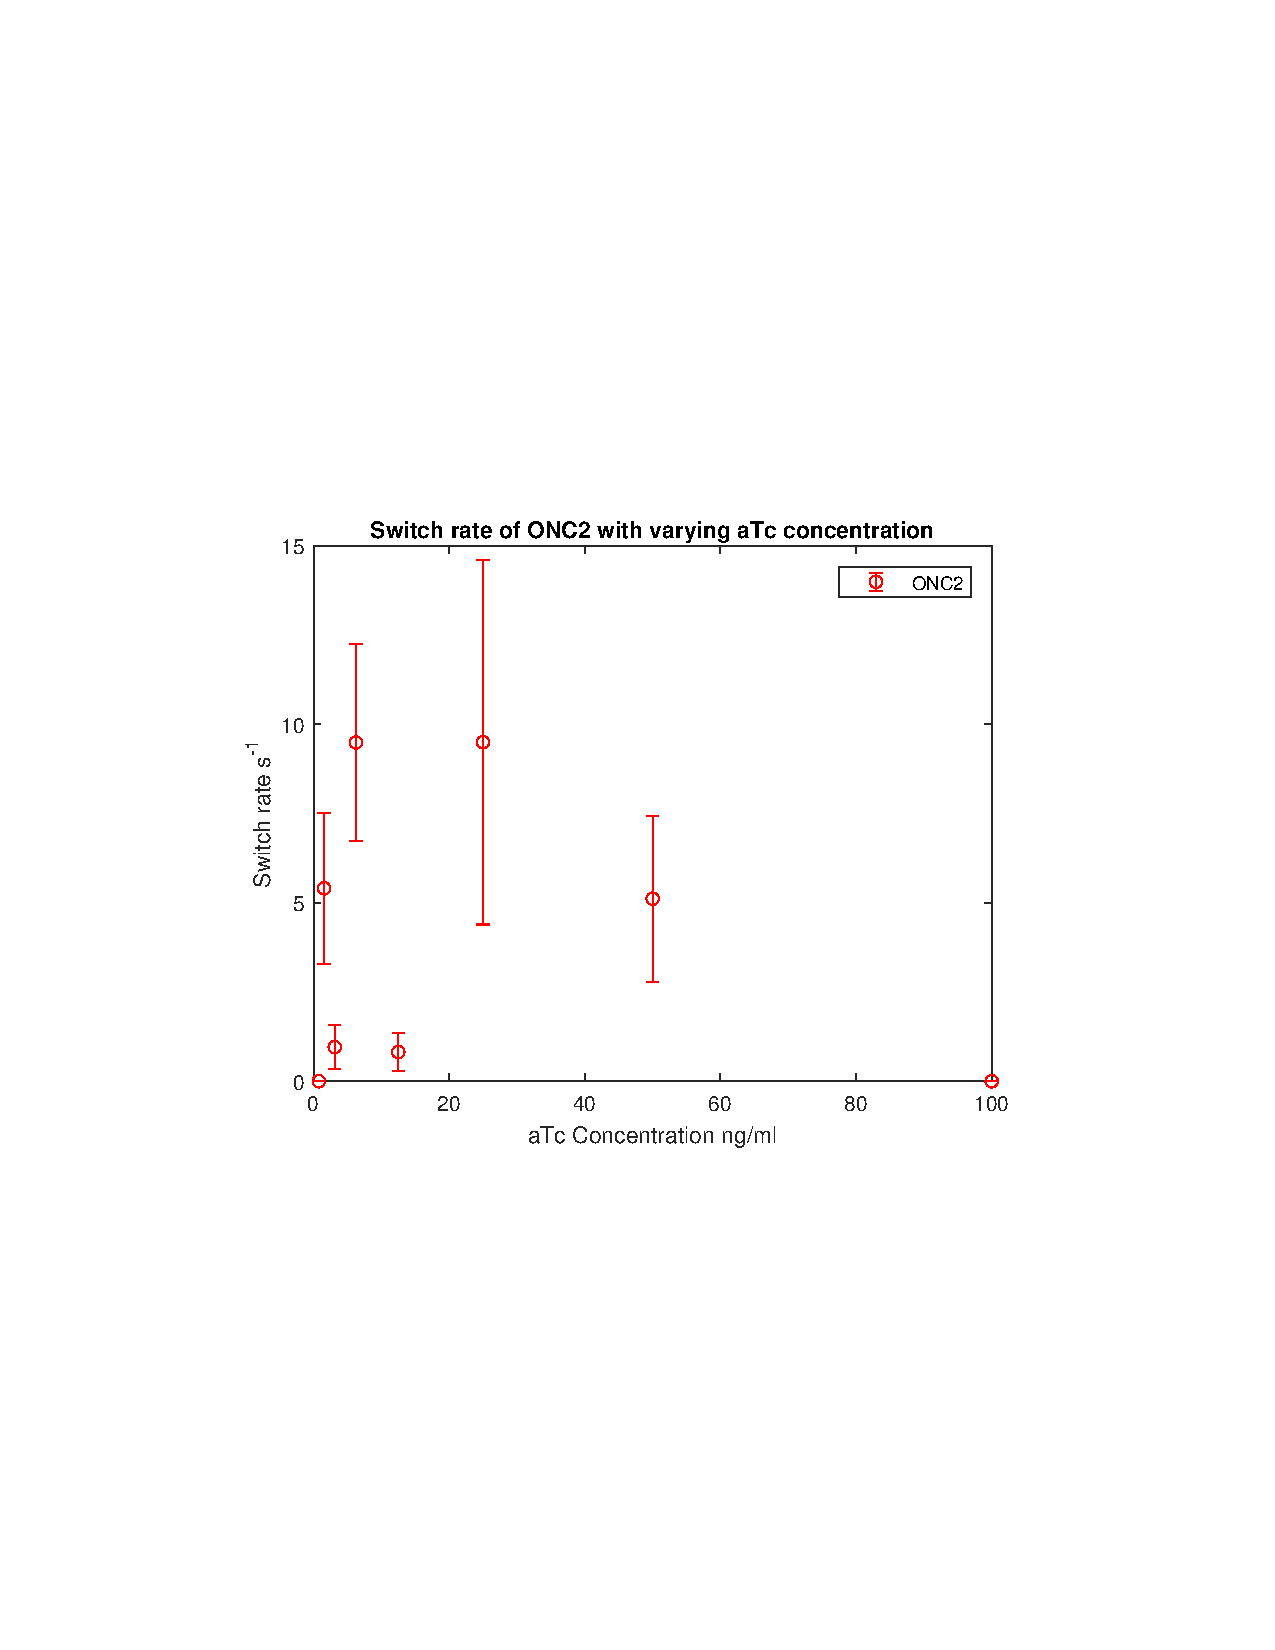
\includegraphics[scale=0.8]{ONC2switchrate.pdf}
\caption{}
\label{fig:onc2SwitchRate}
\end{figure}

Figure \ref{fig:onc1SwitchRate} and \ref{fig:onc2SwitchRate} summarizes the switching rates obtained from the data. 

\pagebreak
\section{Single cell fluorescence}
In this part, we took pictures of several bacteria with a microscope and analyzed them. The goal was to observe the switching of the bacterial states by dint of  GFP and RFP intensities. We used \textit{Fiji}, an image processing software to measure the single cell fluorescence of each bacterium in the image. 

\subsection{Composite images}
The following composite images show the green and red fluorescence intensities of ONC1 and ONC2 in different states. 

%--------------green state------------------
\begin{figure}[h]
\centering
	\begin{minipage}{.5\textwidth}
  		\centering
  		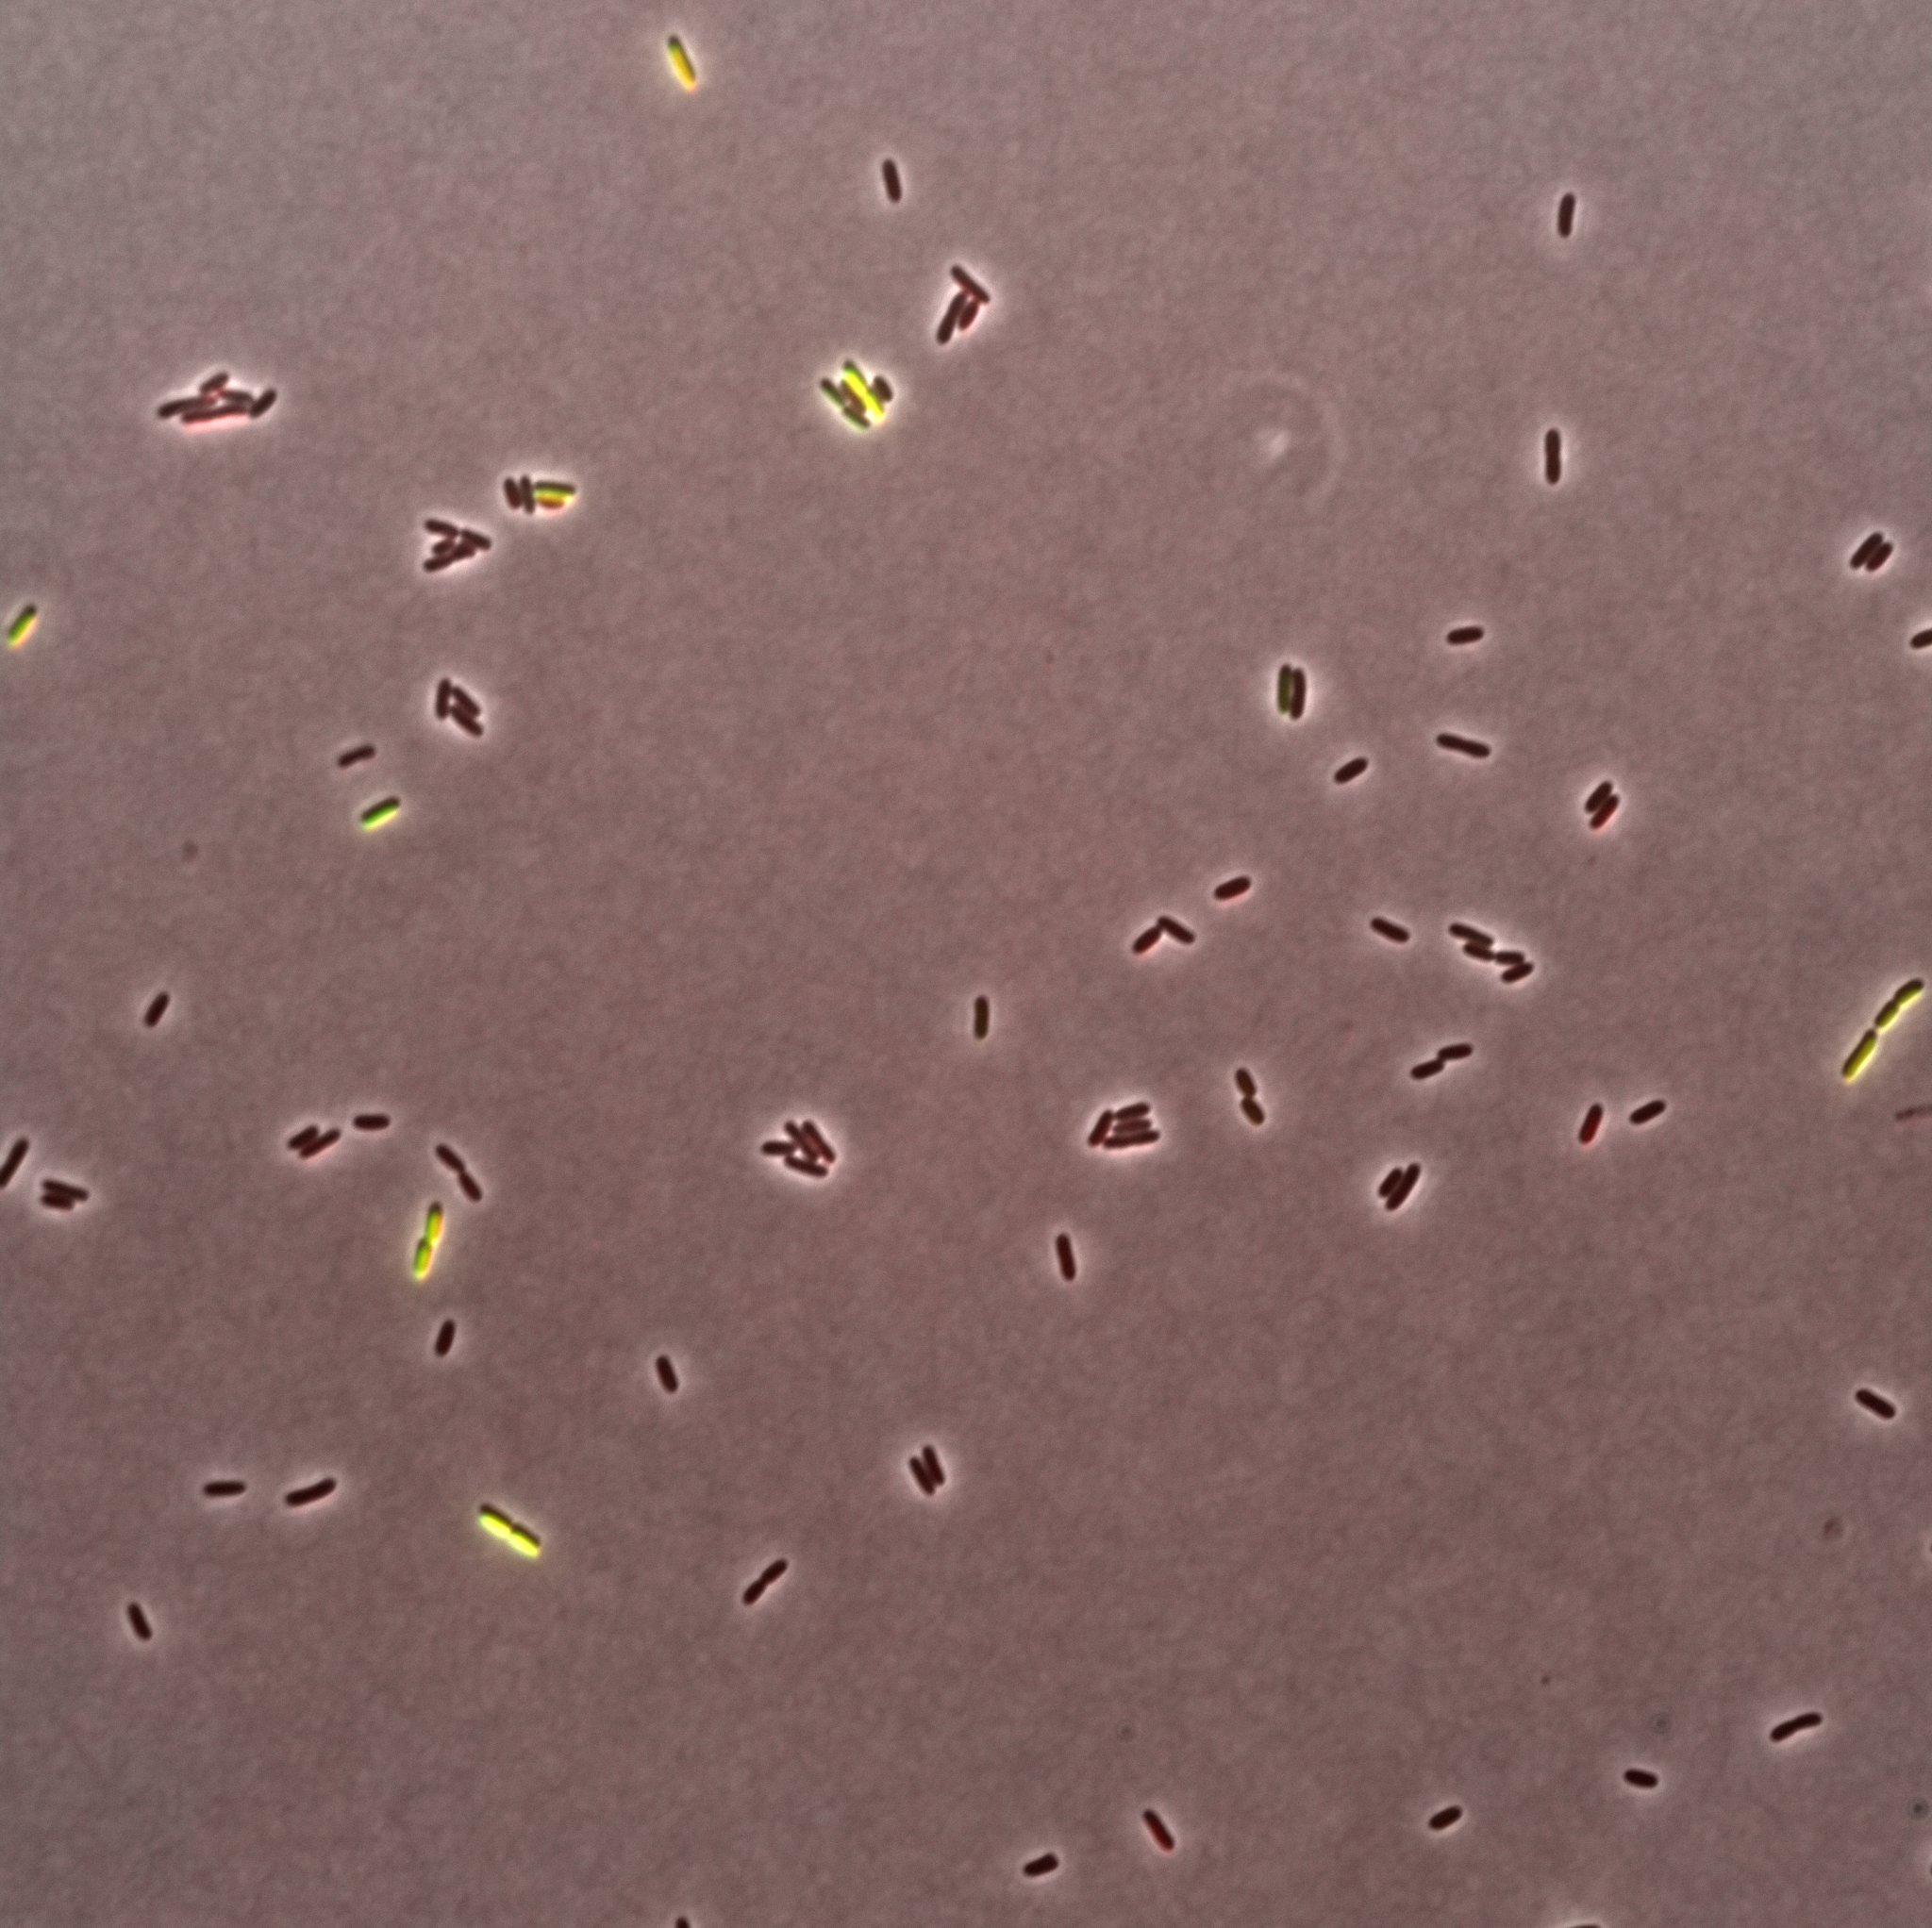
\includegraphics[width=.9\linewidth]{greenstate008Composite.jpg}
  		\captionof{figure}{ONC1 in Green State }
  		\label{fig:onc1GreenStateComposite}
	\end{minipage}%
	\begin{minipage}{.5\textwidth}
  		\centering
  		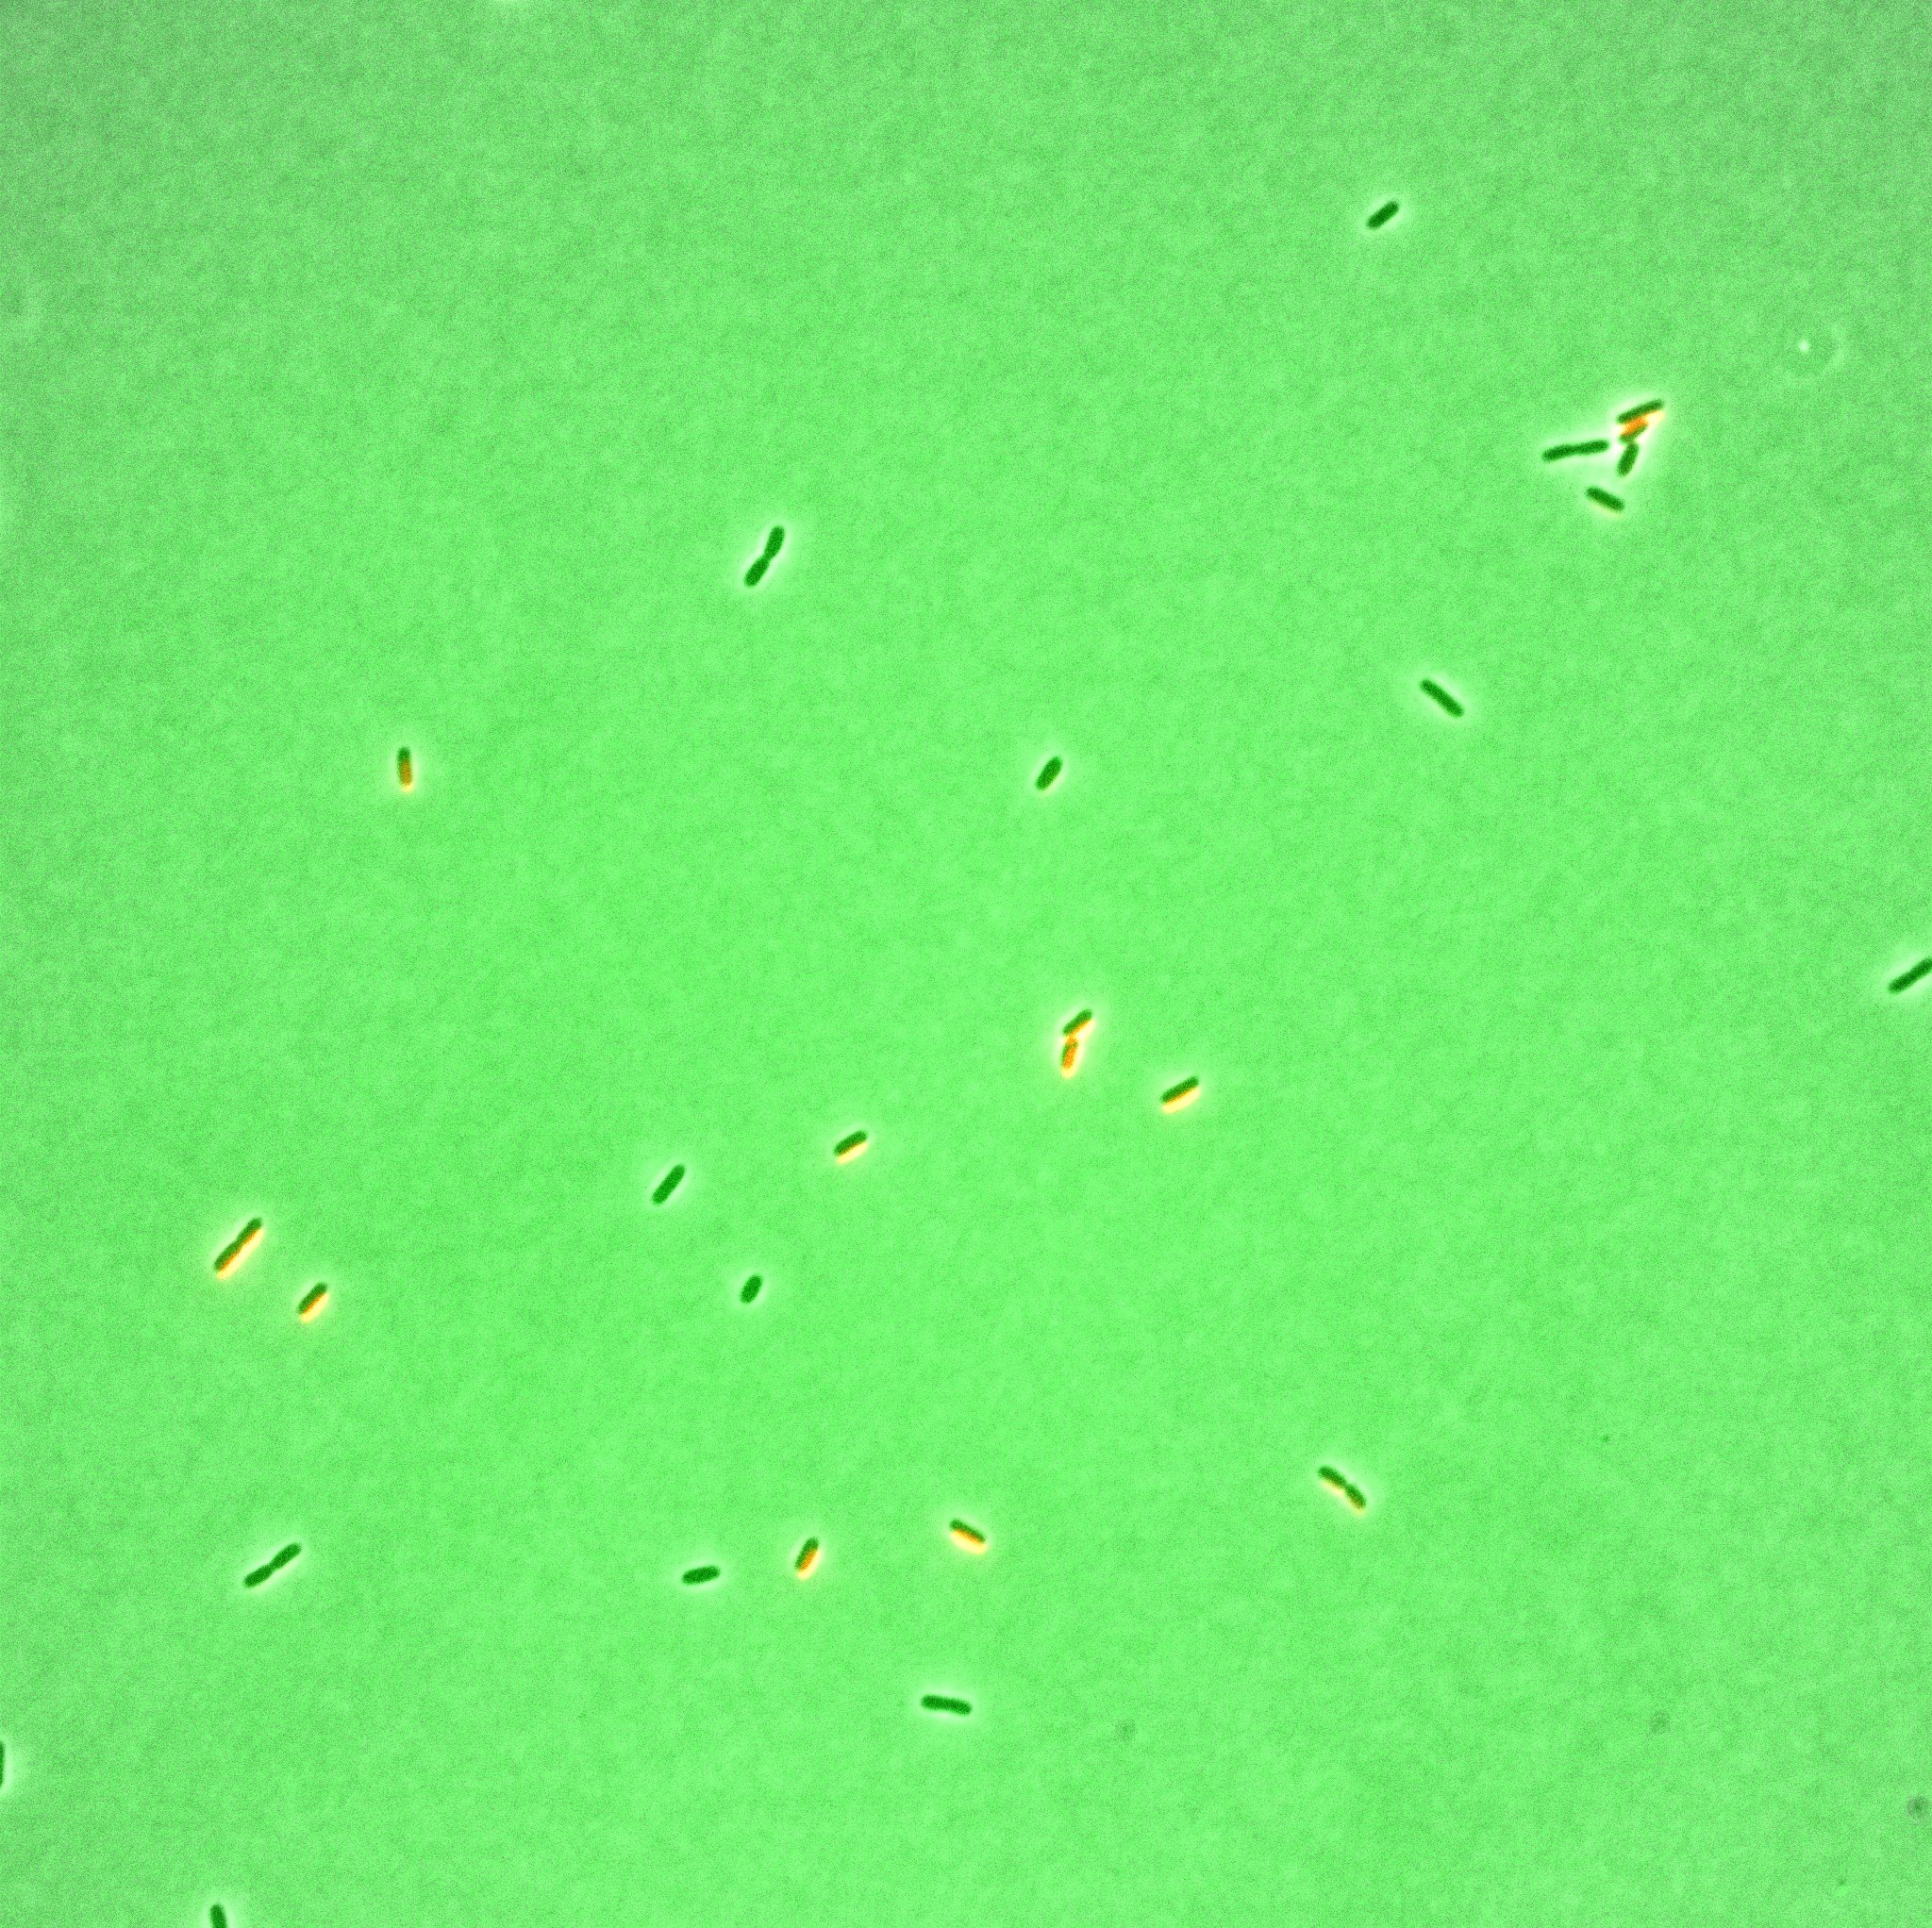
\includegraphics[width=.9\linewidth]{redstate014Composite.jpg}
  		\captionof{figure}{ONC2 in Red State}
  		\label{fig:onc1RedStateComposite}  
	\end{minipage}
\end{figure}

%--------------green state------------------
\begin{figure}
\centering
	\begin{minipage}{.5\textwidth}
  		\centering
  		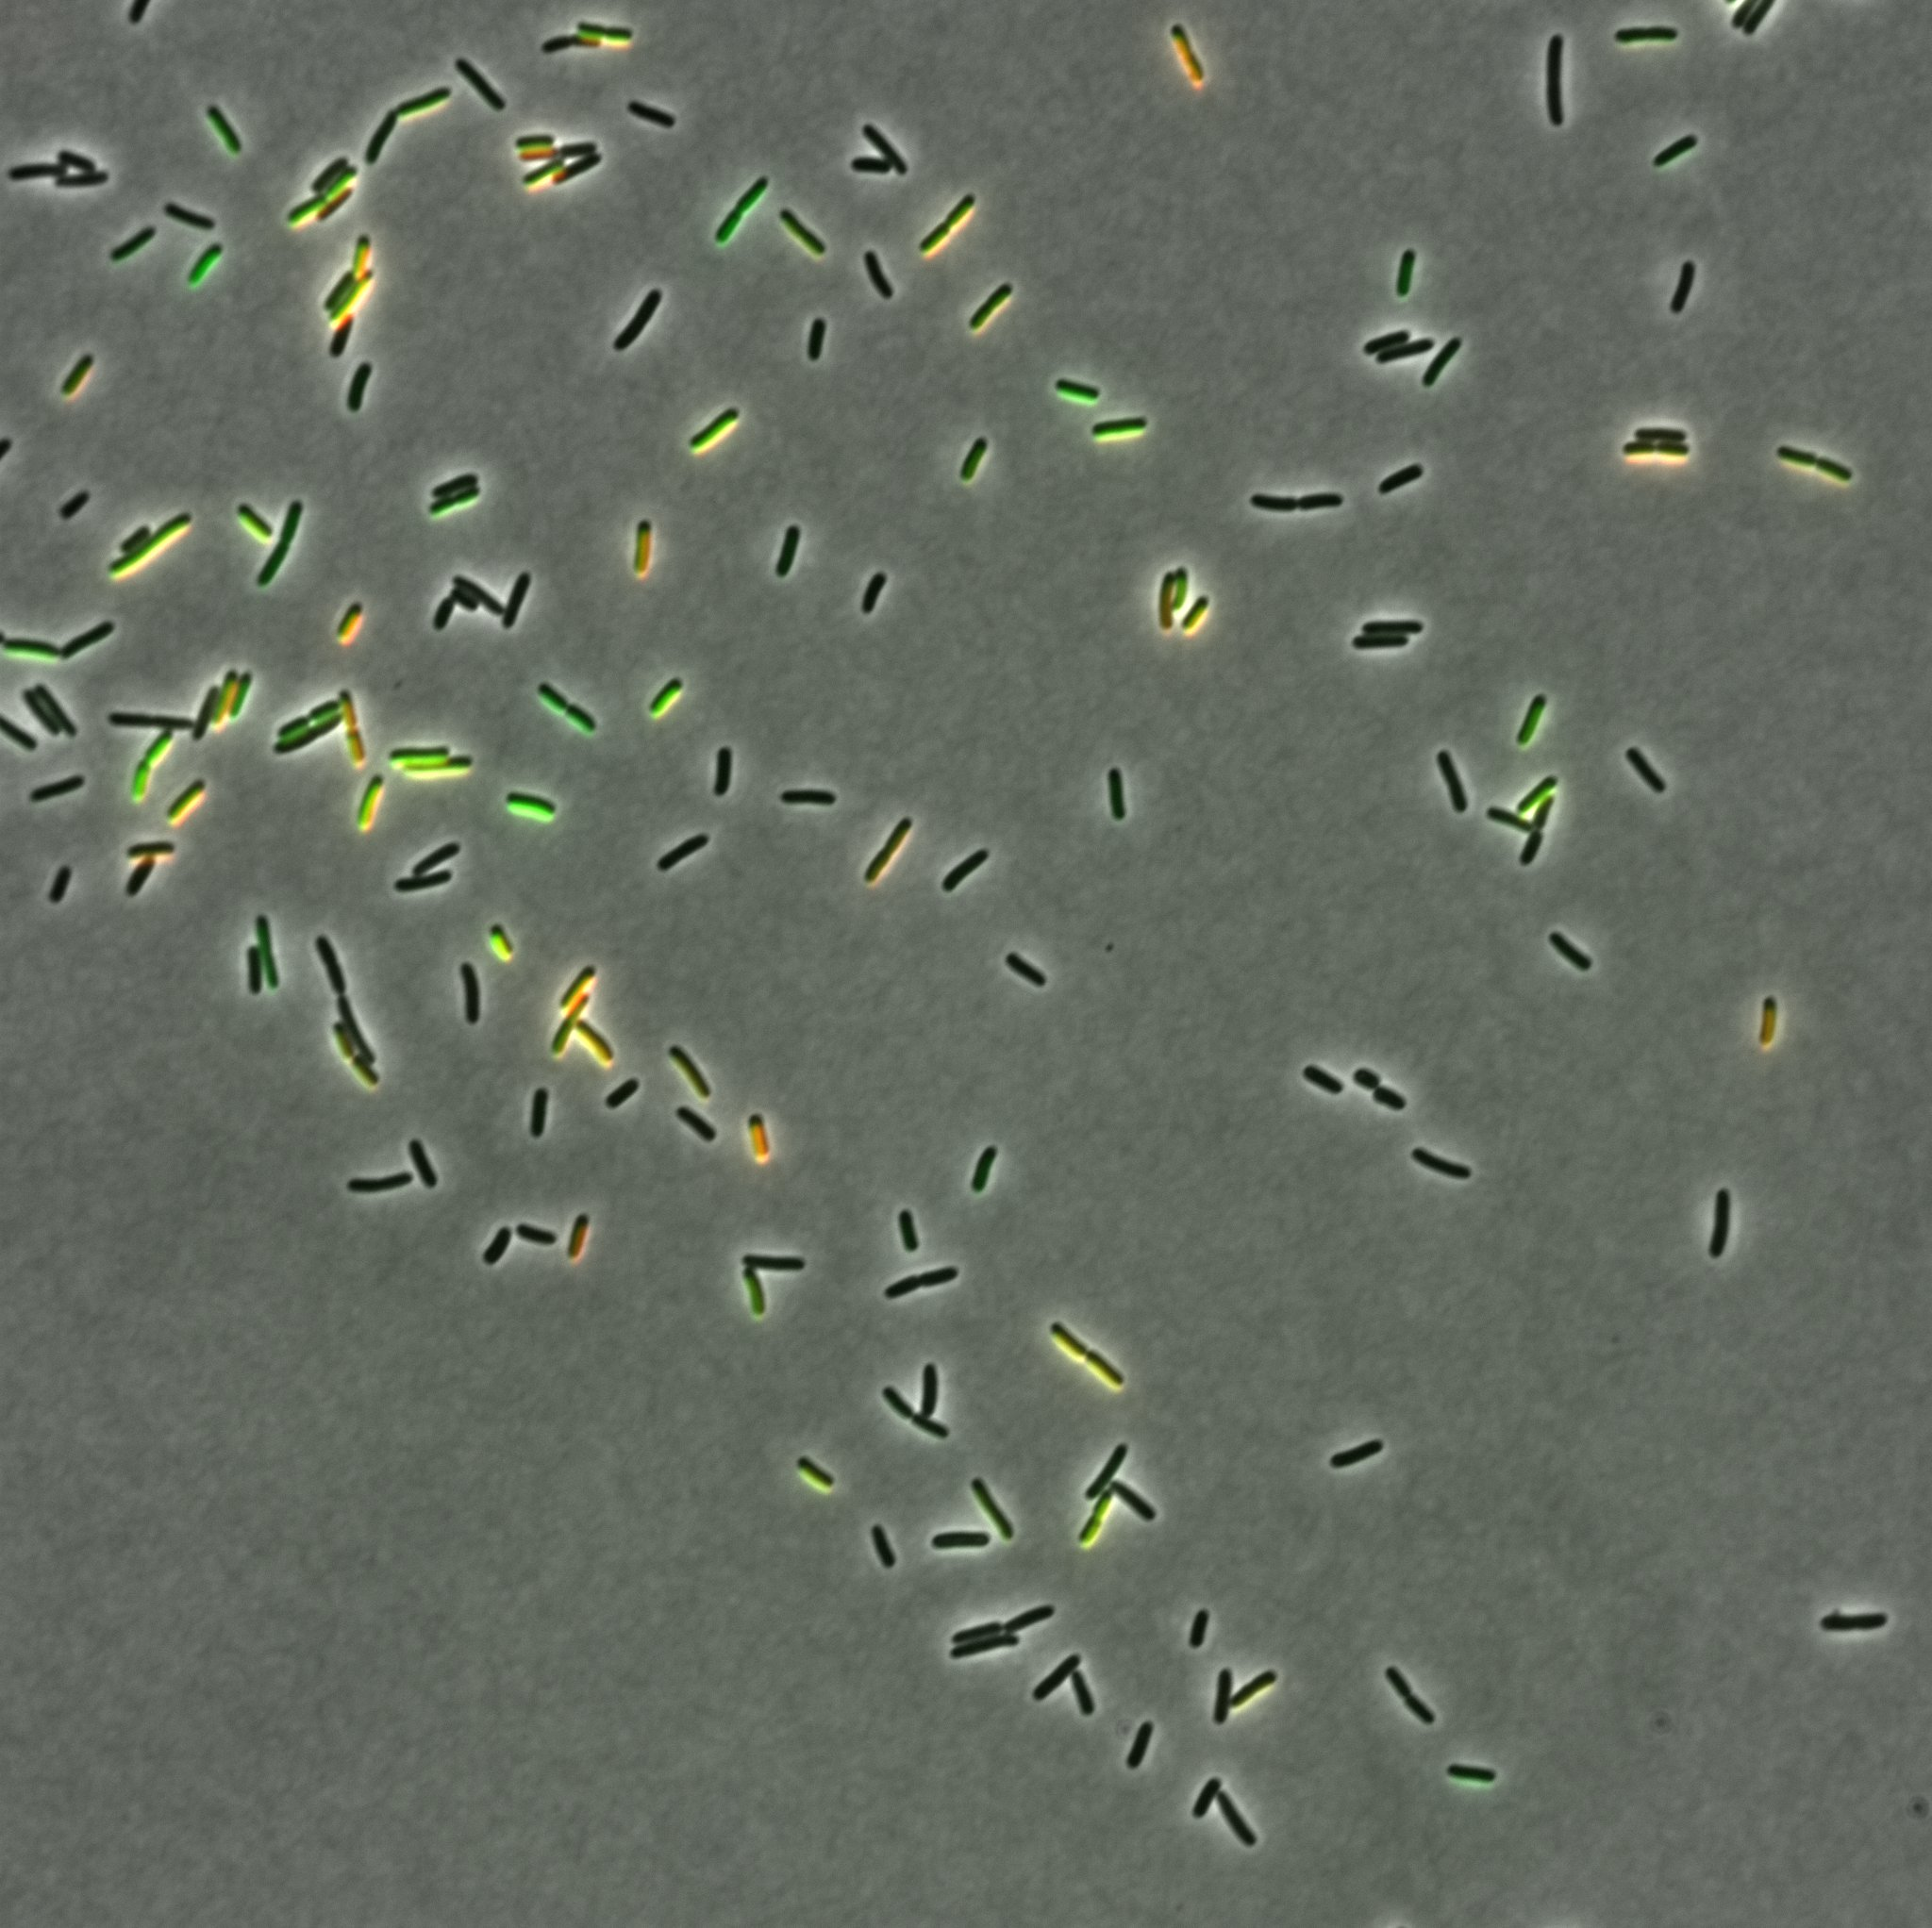
\includegraphics[width=.9\linewidth]{d8007LateComposite.jpg}
  		\captionof{figure}{ONC1 after several hours }
  		\label{fig:onc1AfterHoursComposite}
	\end{minipage}%
	\begin{minipage}{.5\textwidth}
  		\centering
  		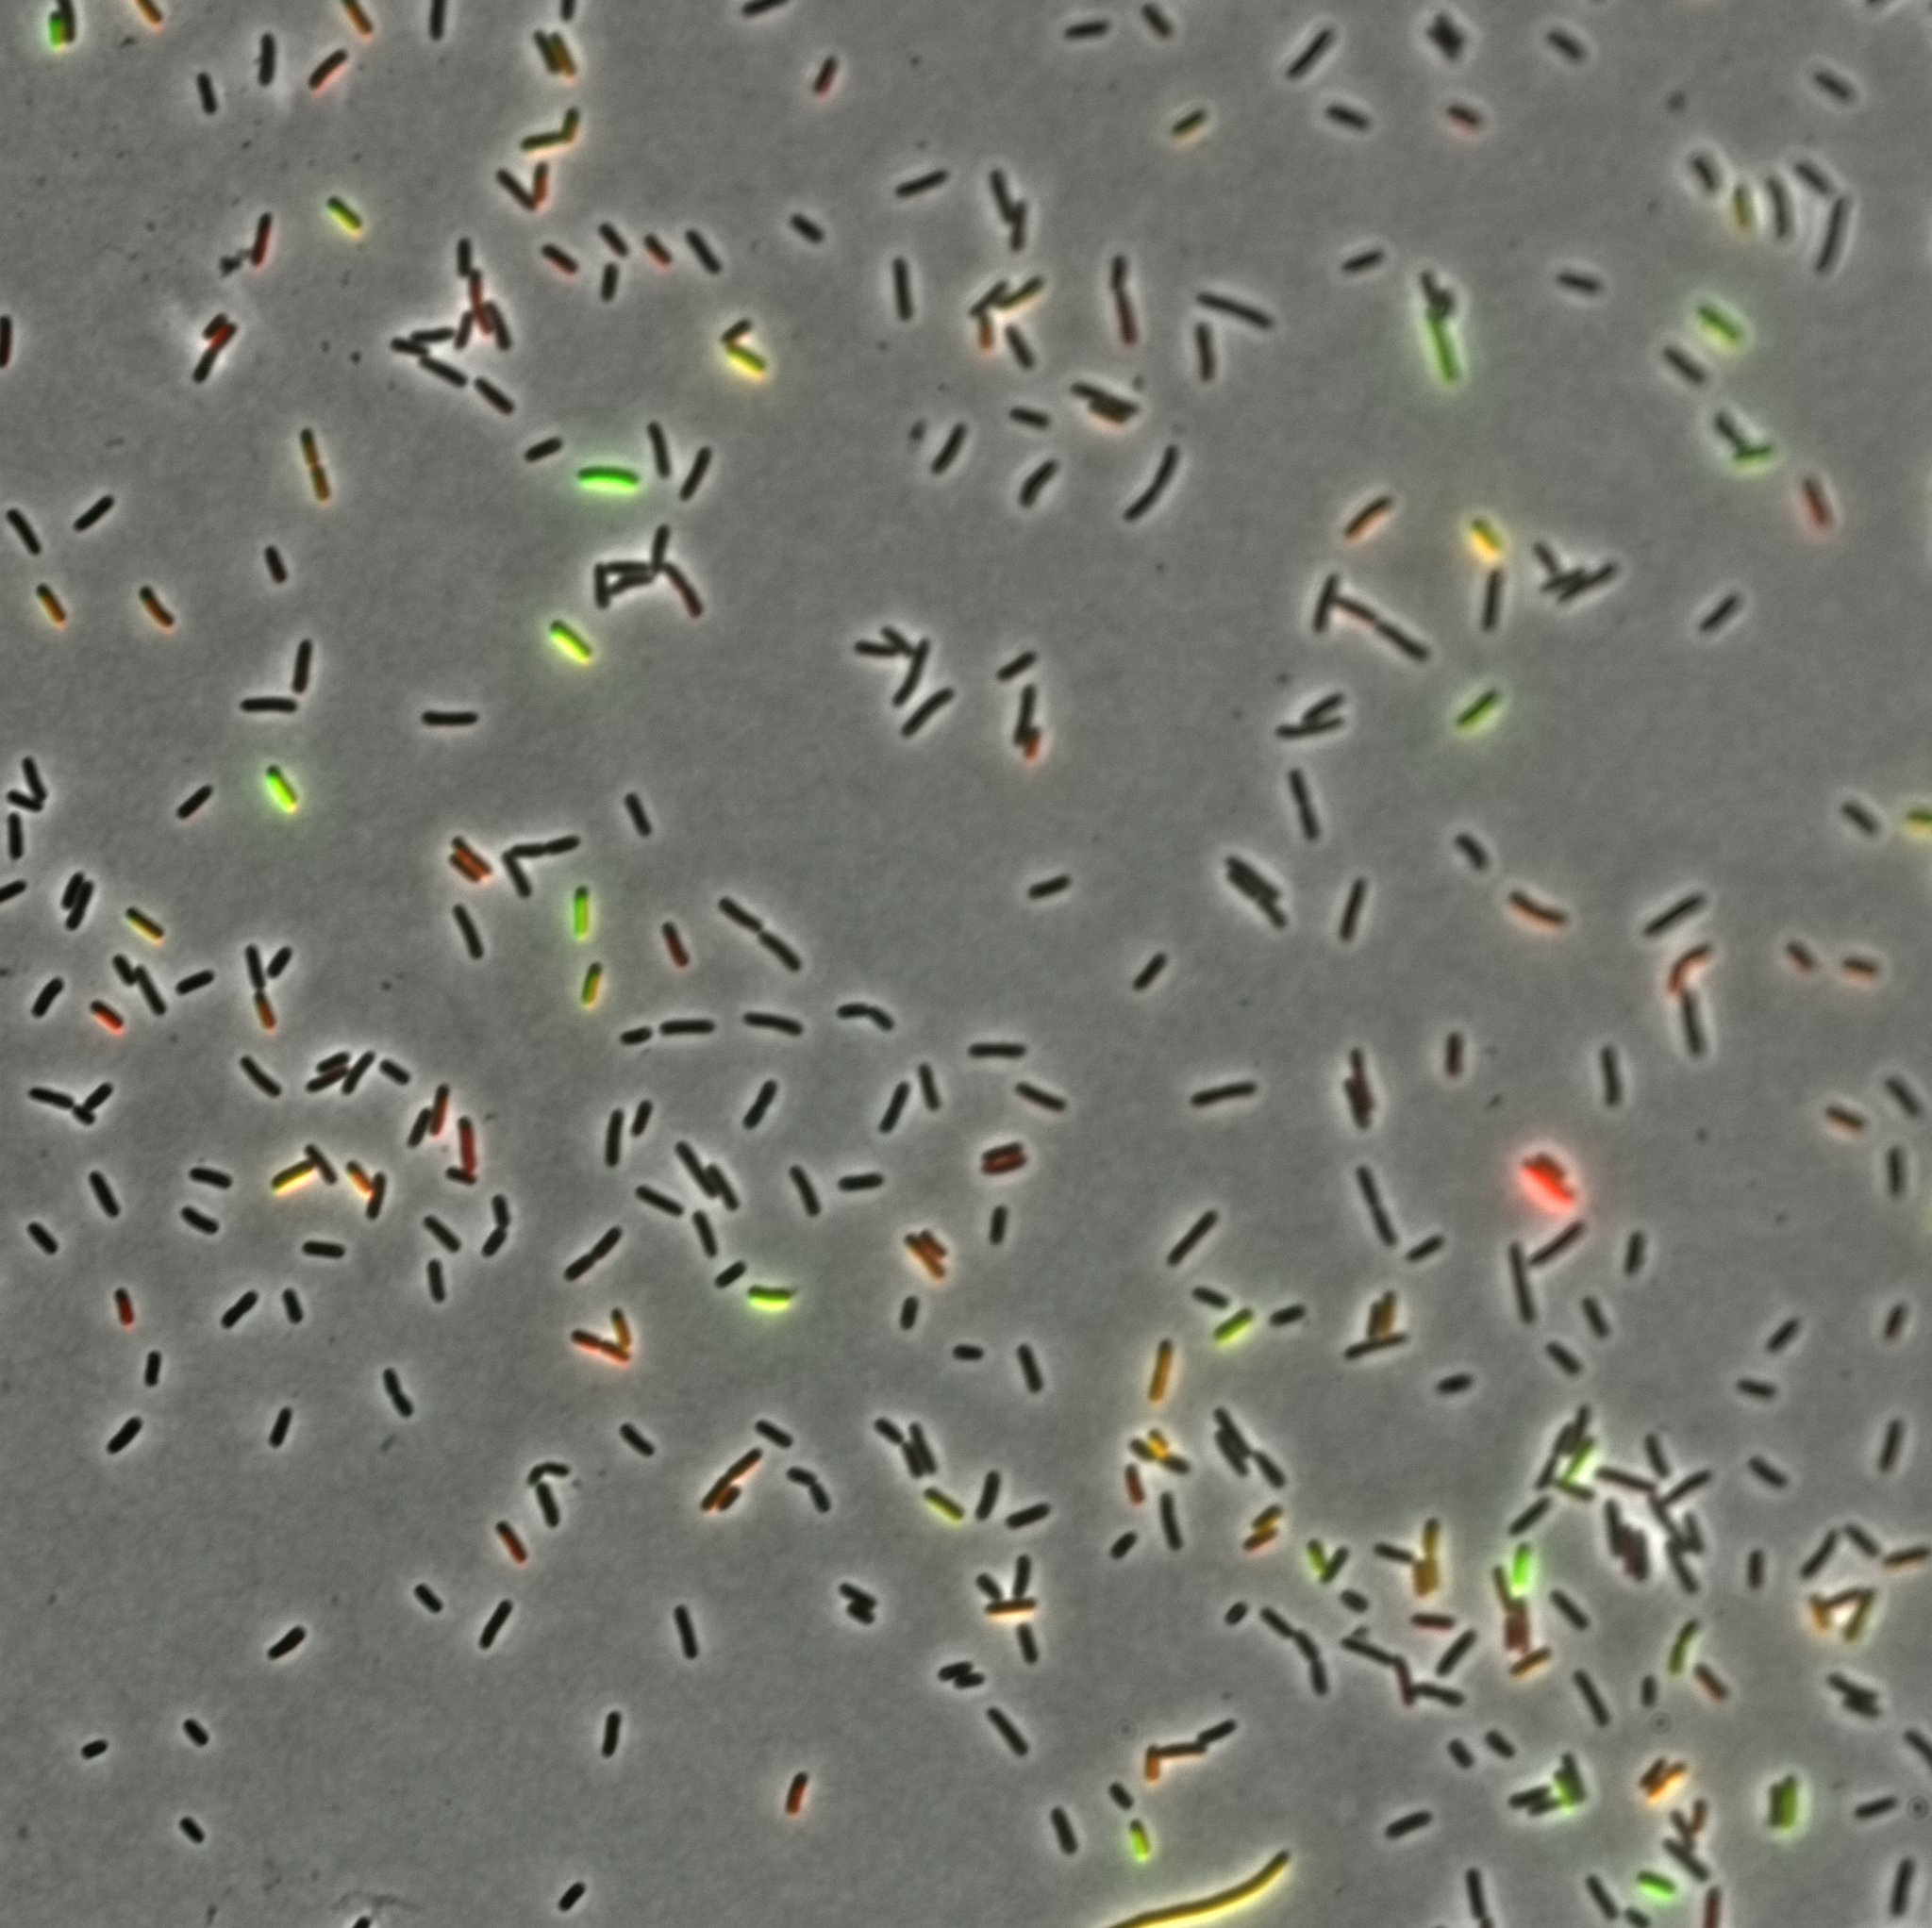
\includegraphics[width=.9\linewidth]{h8LateComposite.jpg}
  		\captionof{figure}{ONC2 after several hours}
  		\label{fig:onc2AfterHoursComposite}  
	\end{minipage}
\end{figure}

At the begining of the experiment, ideally we would expect the ONC1 collection to be completely in green state and the ONC2 in red state. As we can see in the figures \ref{fig:onc1GreenStateComposite} - \ref{fig:onc2AfterHoursComposite}, our samples did not have very strong green and red fluorescence. For the time-evolution, we chose the cultures in the D8 and H8 wells of chart \ref{concGrad}. Both of them were exposed to the highest concentration of IPTG and aTc respectively according to our setup. 

\subsection{Histograms}
According our image analysis data from Fiji, we quantitatively obtained the green and red fluorescence of the cultures in the images. We generated histograms which indicate a frequency distribution of how many bacteria shine how in which states. 

\pagebreak
%--------------green state------------------
\begin{figure}
\centering
	\begin{minipage}{.5\textwidth}
  		\centering
  		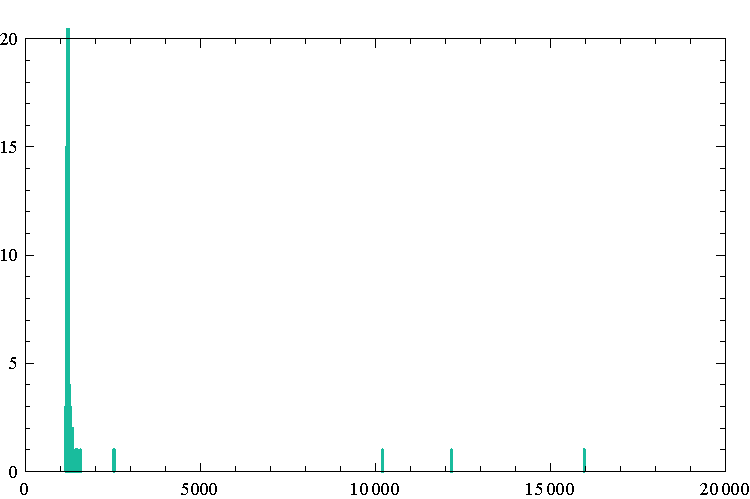
\includegraphics[width=.9\linewidth]{greenstate008GFP.pdf}
  		\captionof{figure}{ONC1 GFP in Green State }
  		\label{fig:onc1GFPGreenState}
	\end{minipage}%
	\begin{minipage}{.5\textwidth}
  		\centering
  		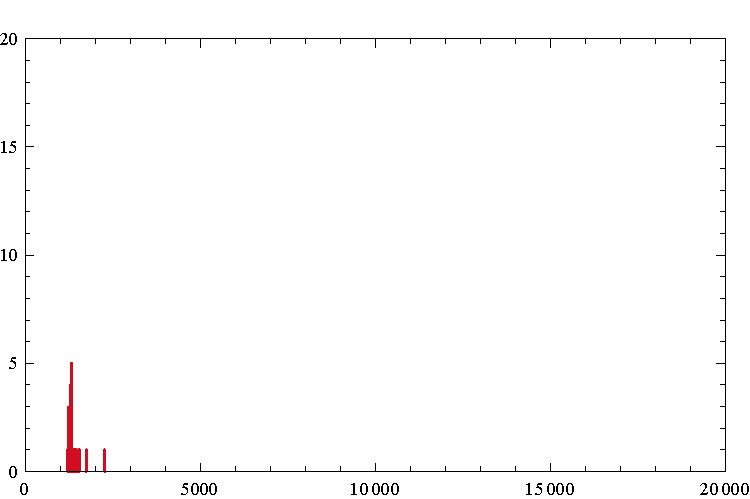
\includegraphics[width=.9\linewidth]{greenstate008RFP.pdf}
  		\captionof{figure}{ONC1 RFP in Green State}
  		\label{fig:onc1RFPGreenState}  
	\end{minipage}
\end{figure}
%--------------red state------------------
\begin{figure}[h]
\centering
	\begin{minipage}{.5\textwidth}
  		\centering
  		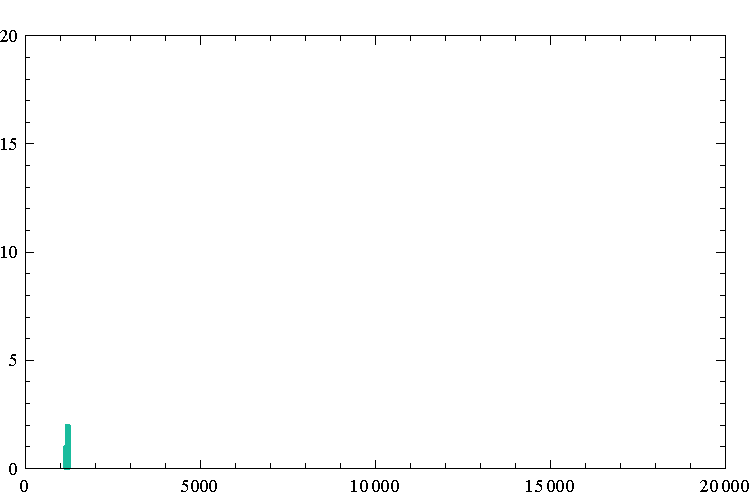
\includegraphics[width=.9\linewidth]{redstate014GFP.pdf}
  		\captionof{figure}{ONC2 GFP in Red State }
  		\label{fig:onc2GFPRedState}
	\end{minipage}%
	\begin{minipage}{.5\textwidth}
  		\centering
  		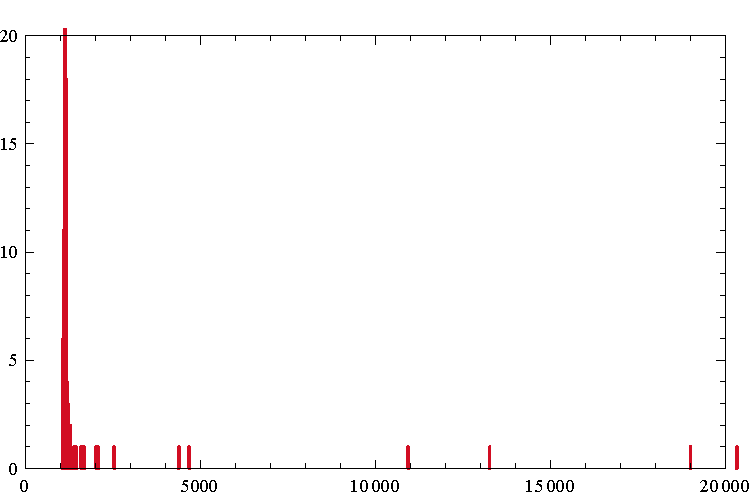
\includegraphics[width=.9\linewidth]{redstate014RFP.pdf}
  		\captionof{figure}{ONC2 RFP in Red State}
  		\label{fig:onc2RFPRedState}  
	\end{minipage}
\end{figure}

%-----green state after time-evolution ------------------
\begin{figure}[h]
\centering
	\begin{minipage}{.5\textwidth}
  		\centering
  		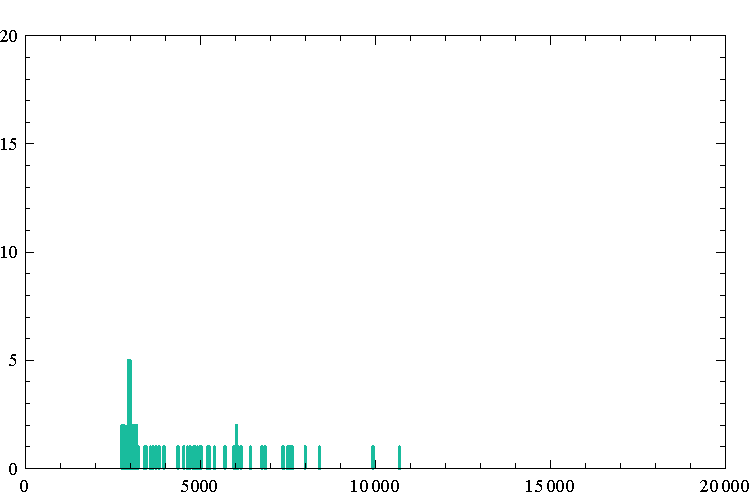
\includegraphics[width=.9\linewidth]{d8007GFP.pdf}
  		\captionof{figure}{ONC1 GFP after several hours }
  		\label{fig:onc1GFPAfterHours}
	\end{minipage}%
	\begin{minipage}{.5\textwidth}
  		\centering
  		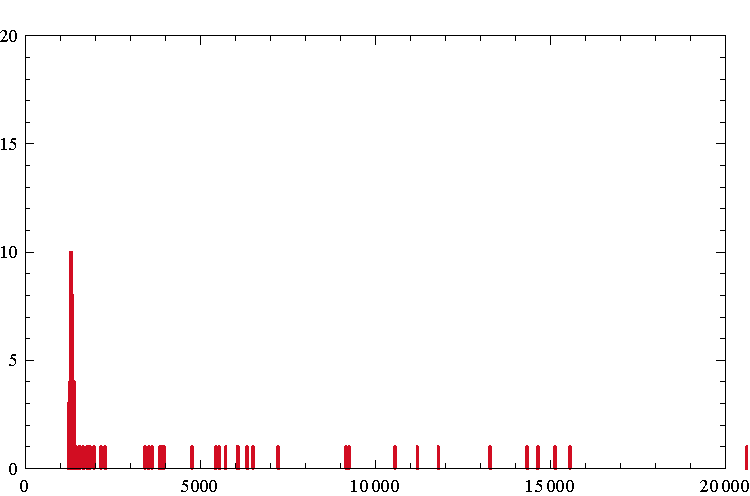
\includegraphics[width=.9\linewidth]{d8007RFP.pdf}
  		\captionof{figure}{ONC1 RFP after several hours}
  		\label{fig:onc1RFPAfterHours}  
	\end{minipage}
\end{figure}

%-----red state after time-evolution ------------------
\begin{figure}[h]
\centering
	\begin{minipage}{.5\textwidth}
  		\centering
  		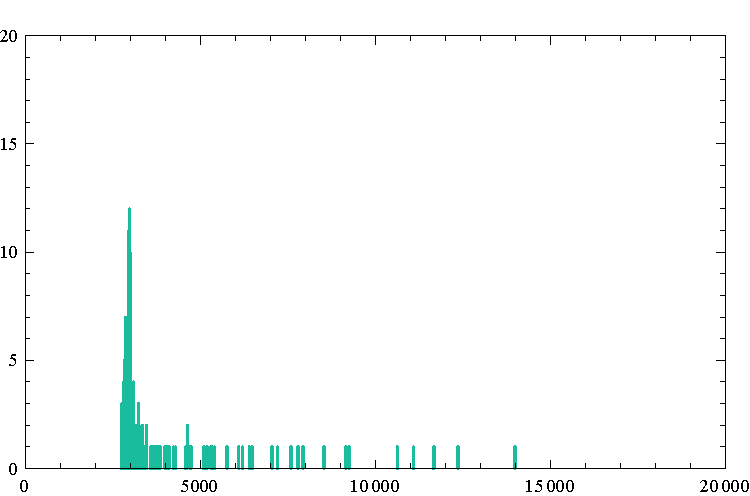
\includegraphics[width=.9\linewidth]{h8LateGFP.pdf}
  		\captionof{figure}{ONC2 GFP after several hours }
  		\label{fig:onc2GFPAfterHours}
	\end{minipage}%
	\begin{minipage}{.5\textwidth}
  		\centering
  		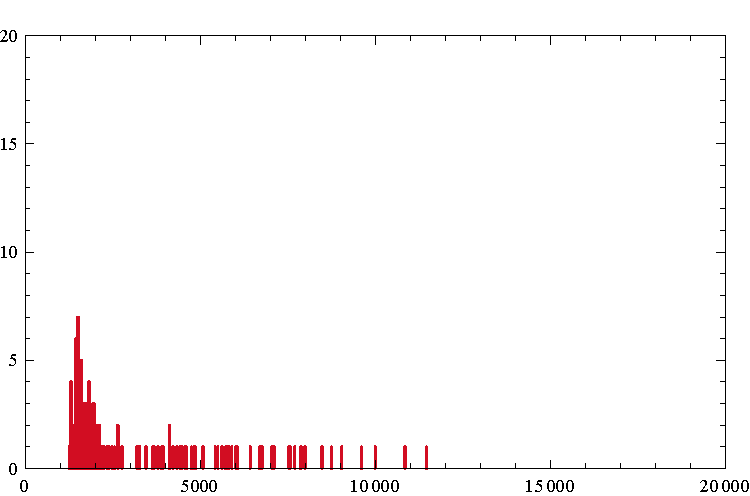
\includegraphics[width=.9\linewidth]{h8LateRFP.pdf}
  		\captionof{figure}{ONC2 RFP after several hours}
  		\label{fig:onc2RFPAfterHours}  
	\end{minipage}
\end{figure}

The first four histograms in the figures \ref{fig:onc1GFPGreenState} - \ref{fig:onc2RFPRedState} show that, most of the  ONC1 bacteria in green state have the high GFP intensity, and ONC2 bacteria have high RFP intensity, as expected. If switching happens, then over a time evolution we would expect the green-state cultures to lose their GFP intensities and red-state cultures to lose their RFP intensities.

The Last four histograms (figures \ref{fig:onc1GFPAfterHours} - \ref{fig:onc2RFPAfterHours}) show that the ONC1 bacteria indeed started losing GFP intensity and gaining the RFP intensity. The opposite happened with the ONC2. So, we can say that the switching started to take place, but was not complete when we reached the end of the experiment. 

\subsection{Switching rate}
Our observation presents the following result

\begin{table}[h]
\centering
\label{switchingRateTable}
\begin{tabular}{lllll}
 	At beginning &  ONC1 &  in Green state	&  97.9730\% $\pm 1\%$ &  \\
	After 4 hrs	 &  ONC1 &  in Green State 	&  61.6279\% $\pm 1\%$ &  \\
	At beginning &  ONC2 &  in Red State	&  92.9134\% $\pm 1\%$ &  \\
	After 4 hrs	 &  ONC2 &  in Red State 	&  80.1762\% $\pm 1\%$ &  \\
\end{tabular}
\caption{Observation of switching}
\end{table}

Hence, approximately $9.1\%$ bacteria switch from Green to Red state in ONC1, and approximately $3.2\%$ bacteria switch from Red to Green state in ONC2. 



\pagebreak
\chapter{Appendix}

\begin{figure}[h]
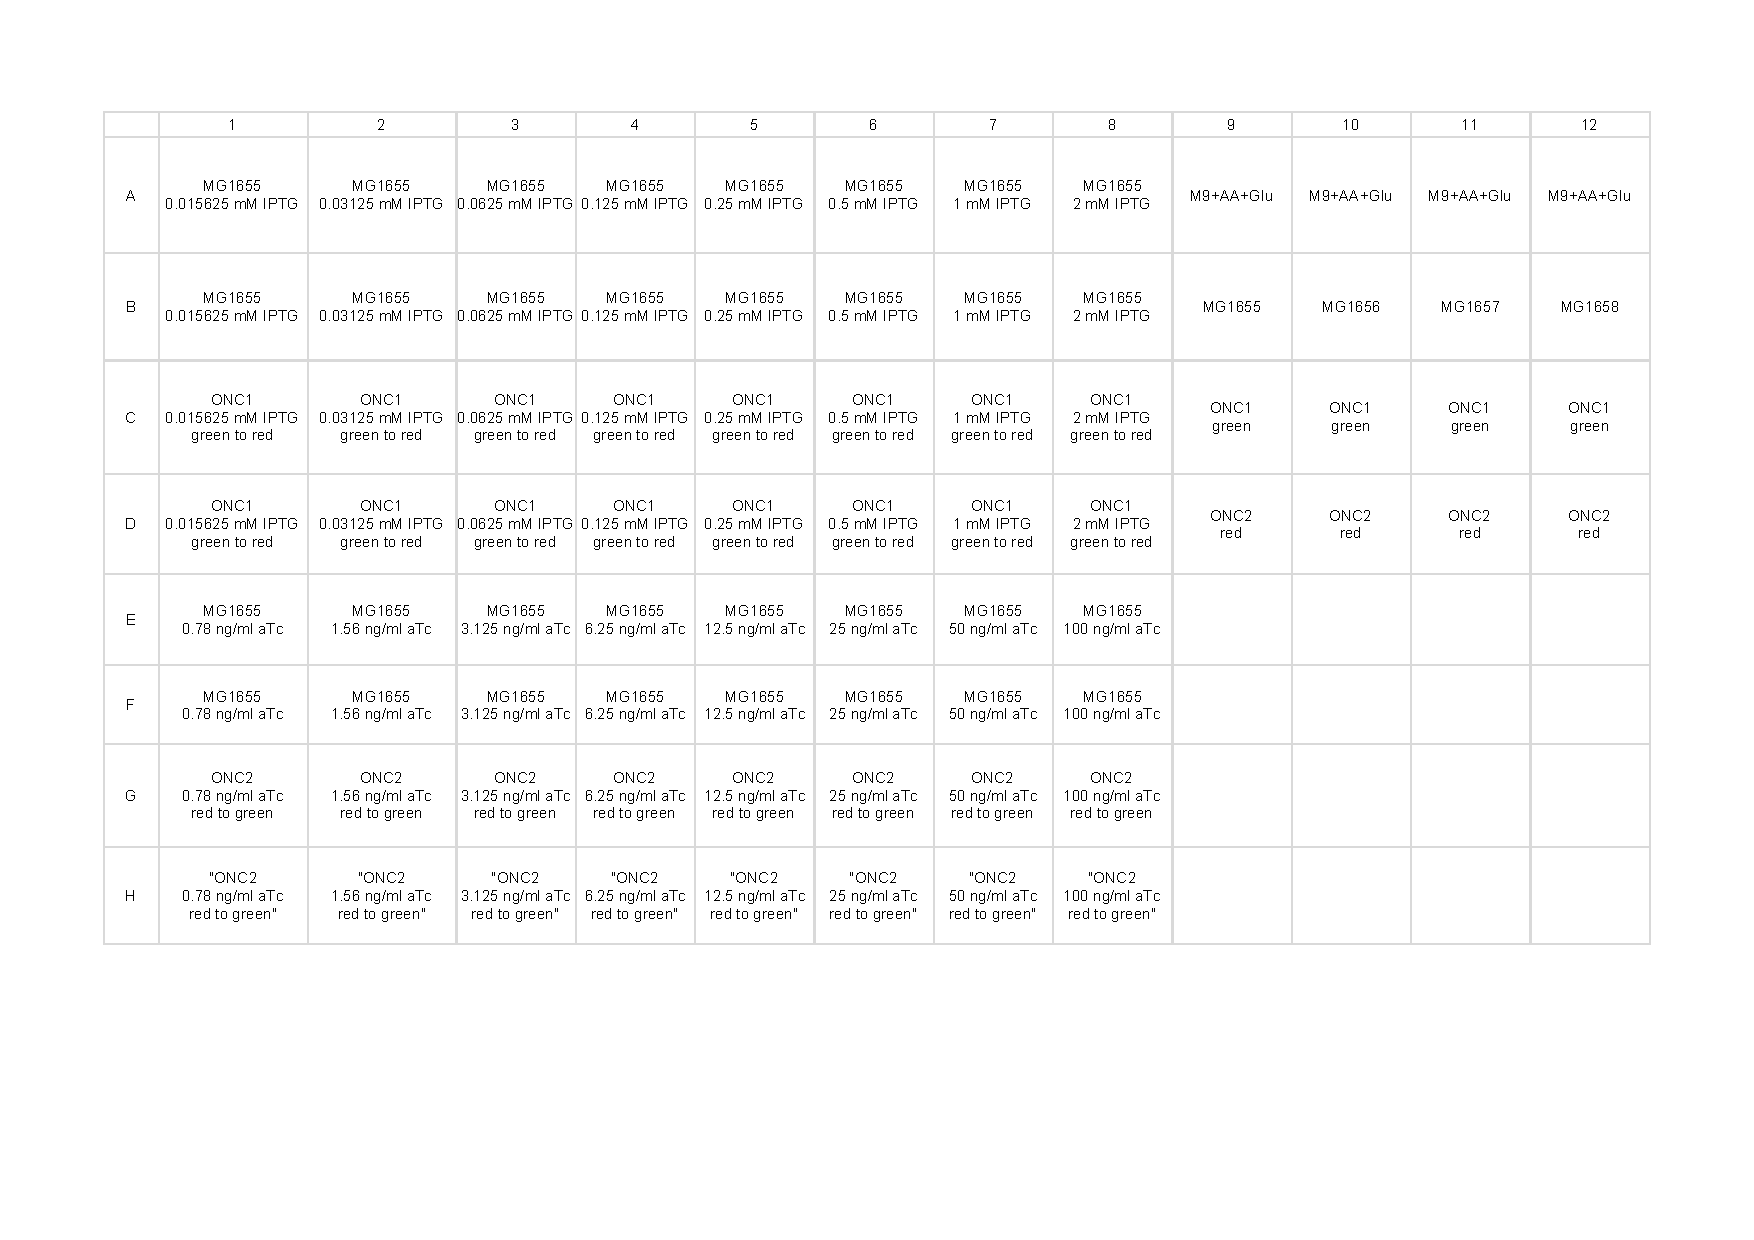
\includegraphics[scale=0.8, angle=-90, origin=c]{concentrationGradient}
\caption{Concentration gradient of IPTG and aTc}
\label{concGrad}
\end{figure}

\pagebreak

\begin{figure}[h]
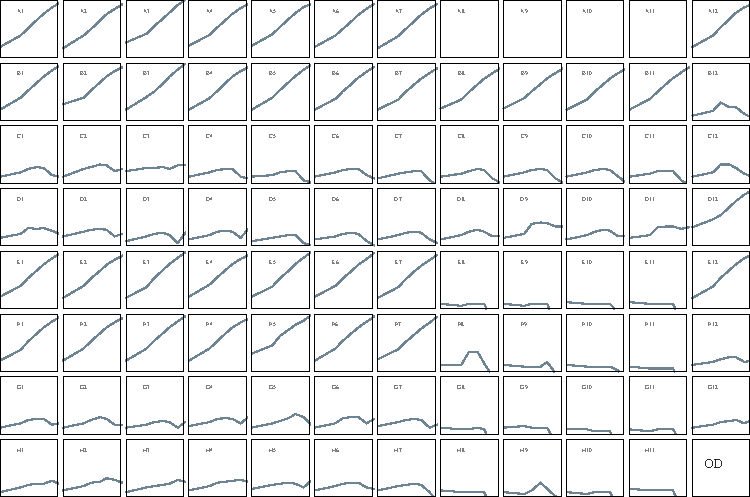
\includegraphics[scale=1.7, angle=-90, origin=c]{OD-LogPlot.pdf}
\caption{
Optical Density of each well in figure \ref{concGrad} (measured over time from 0 to 14000 seconds in horizontal axes). The Vertical axes are logarithmic.}
\label{ODLogPlot}
\end{figure}


\begin{figure}[h]
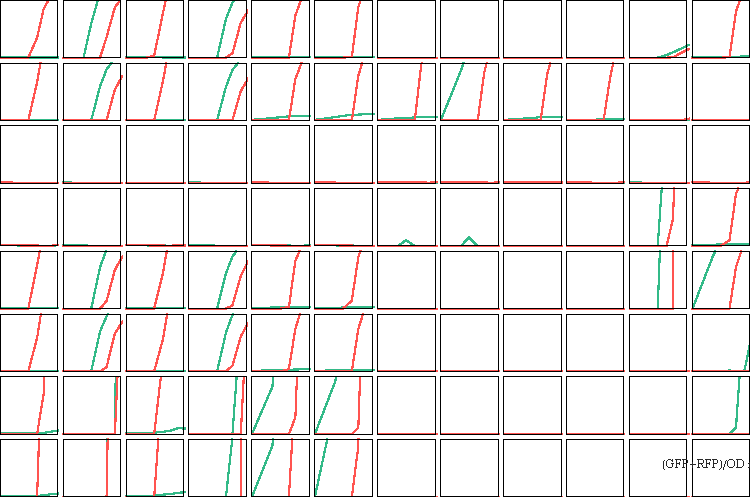
\includegraphics[scale=1.7, angle=-90, origin=c]{GfpPlusRfpByODCorrectedYMax80000.pdf}
\caption{
GFP/OD and RFP/OD. over time. The Vertical axes are logarithmic.}
\label{fig:GfpRfpByOD}
\end{figure}

-

\pagebreak

\begin{figure}[h]
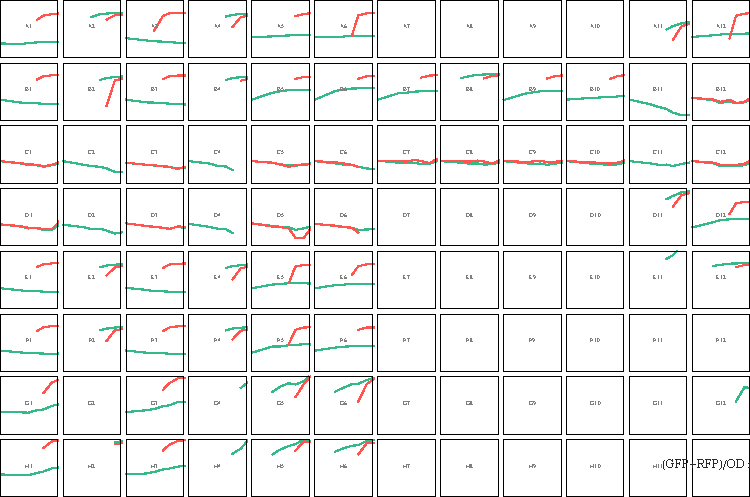
\includegraphics[scale=1.7, angle=-90, origin=c]{LogGfpPlusRfpByODCorrectedYMax12.pdf}
\caption{
GFP/OD and RFP/OD. over time. The Vertical axes are logarithmic.}
\label{fig:GfpRfpByODLog}
\end{figure}



\end{document}